%----------------------------------------------------------------------------------------
%	PACKAGES AND OTHER DOCUMENT CONFIGURATIONS
%----------------------------------------------------------------------------------------

\documentclass{article}

\usepackage{fancyhdr} % Required for custom headers
\usepackage{lastpage} % Required to determine the last page for the footer
\usepackage{extramarks} % Required for headers and footers
\usepackage[usenames,dvipsnames]{color} % Required for custom colors
\usepackage{graphicx} % Required to insert images
\usepackage{listings} % Required for insertion of code
\usepackage{courier} % Required for the courier font
\usepackage{lipsum} % Used for inserting dummy 'Lorem ipsum' text into the template
\usepackage{parskip}
% Margins
\topmargin=-0.45in
\evensidemargin=0in
\oddsidemargin=0in
\textwidth=6.5in
\textheight=9.0in
\headsep=0.25in

\usepackage{pdfpages}

\linespread{1.1} % Line spacing

% Set up the header and footer
\pagestyle{fancy}
\chead{} % Top left header
\lhead{\hmwkClass\  \hmwkTitle} % Top center head
\rhead{} % Top right header
\lfoot{\lastxmark} % Bottom left footer
\cfoot{} % Bottom center footer
\rfoot{Page\ \thepage\ of\ \protect\pageref{LastPage}} % Bottom right footer
\renewcommand\headrulewidth{0.4pt} % Size of the header rule
\renewcommand\footrulewidth{0.4pt} % Size of the footer rule

\setlength\parindent{0pt} % Removes all indentation from paragraphs

%----------------------------------------------------------------------------------------
%	CODE INCLUSION CONFIGURATION
%----------------------------------------------------------------------------------------

% \definecolor{MyDarkGreen}{rgb}{0.0,0.4,0.0} % This is the color used for comments
\lstloadlanguages{C} % Load C syntax for listings, for a list of other languages supported see: ftp://ftp.tex.ac.uk/tex-archive/macros/latex/contrib/listings/listings.pdf
\lstset{language=C,commentstyle=\color{Green},frame=single,keywordstyle=[1]\color{Blue}\bf} % Use C in this example      



\newcommand{\csnippet}[2]{
\begin{itemize}
\item[]\lstinputlisting[caption=#2,label=#1]{#1.c}
\end{itemize}
}

%----------------------------------------------------------------------------------------
%	DOCUMENT STRUCTURE COMMANDS
%----------------------------------------------------------------------------------------

% Header and footer for when a page split occurs within a problem environment
\newcommand{\enterProblemHeader}[1]{
\nobreak\extramarks{#1}{#1 continued on next page\ldots}\nobreak
\nobreak\extramarks{#1 (continued)}{#1 continued on next page\ldots}\nobreak
}

% Header and footer for when a page split occurs between problem environments
\newcommand{\exitProblemHeader}[1]{
\nobreak\extramarks{#1 (continued)}{#1 continued on next page\ldots}\nobreak
\nobreak\extramarks{#1}{}\nobreak
}

\setcounter{secnumdepth}{0} % Removes default section numbers
\newcounter{homeworkProblemCounter} % Creates a counter to keep track of the number of problems

\newcommand{\homeworkProblemName}{}
\newenvironment{homeworkProblem}[1][Problem \arabic{homeworkProblemCounter}]{ % Makes a new environment called homeworkProblem which takes 1 argument (custom name) but the default is "Problem #"
\stepcounter{homeworkProblemCounter} % Increase counter for number of problems
\renewcommand{\homeworkProblemName}{#1} % Assign \homeworkProblemName the name of the problem
\section{\homeworkProblemName} % Make a section in the document with the custom problem count
\enterProblemHeader{\homeworkProblemName} % Header and footer within the environment
}{
\exitProblemHeader{\homeworkProblemName} % Header and footer after the environment
}

\newcommand{\problemAnswer}[1]{ % Defines the problem answer command with the content as the only argument
\noindent\framebox[\columnwidth][c]{\begin{minipage}{0.98\columnwidth}#1\end{minipage}} % Makes the box around the problem answer and puts the content inside
}

\newcommand{\homeworkSectionName}{}
\newenvironment{homeworkSection}[1]{ % New environment for sections within homework problems, takes 1 argument - the name of the section
\renewcommand{\homeworkSectionName}{#1} % Assign \homeworkSectionName to the name of the section from the environment argument
\subsection{\homeworkSectionName} % Make a subsection with the custom name of the subsection
\enterProblemHeader{\homeworkProblemName\ [\homeworkSectionName]} % Header and footer within the environment
}{
\enterProblemHeader{\homeworkProblemName} % Header and footer after the environment
}

%----------------------------------------------------------------------------------------
%	NAME AND CLASS SECTION
%----------------------------------------------------------------------------------------

\newcommand{\hmwkTitle}{Assignment\ \#5} % assignment title
\newcommand{\hmwkDueDate}{Monday,\ December\ 18,\ 2014} % due date
\newcommand{\hmwkClass}{Programming Concurrent Systems} % class
\newcommand{\hmwkClassTime}{} % lecture time
\newcommand{\hmwkClassInstructor}{} % lecturer
\newcommand{\hmwkAuthorName}{Alyssa - Ilias} %name

%----------------------------------------------------------------------------------------
%	TITLE PAGE
%----------------------------------------------------------------------------------------

\title{
\vspace{2in}
\textmd{\textbf{\hmwkClass:\ \hmwkTitle}}\\
\normalsize\vspace{0.1in}\small{Due\ on\ \hmwkDueDate}\\
\vspace{0.1in}\large{\textit{\hmwkClassInstructor\ \hmwkClassTime}}
\vspace{3in}
}

\author{\textbf{\hmwkAuthorName}}


%----------------------------------------------------------------------------------------

\begin{document}

\maketitle

%----------------------------------------------------------------------------------------
%	TABLE OF CONTENTS
%----------------------------------------------------------------------------------------

%\setcounter{tocdepth}{1} % Uncomment this line if you don't want subsections listed in the ToC

%\newpage
%\tableofcontents
\newpage

%----------------------------------------------------------------------------------------
%	Introduction
%----------------------------------------------------------------------------------------
\begin{homeworkProblem}[Introduction]

This assignment asked us to implement heat dissipation in Chapel and perform comparison experiments
with our previous implementations, and then to experiment further with distributed arrays (using
domain maps) and more low-level distributed methods.


\end{homeworkProblem}
%----------------------------------------------------------------------------------------
%	Heat
%----------------------------------------------------------------------------------------

% To have just one problem per page, simply put a \clearpage after each problem

\begin{homeworkProblem}[Heat dissipation | Chapel]
\textbf{Solution description}

Our Chapel implementation is a pretty straightforward translation of the C reference 
code. The interesting parts are the code segments which are parallelized by Chapel.

First, let's inspect the main computation loop:

We used the forall keyword to indicate that we want the outer loop parallelized. We also tried
using one forall ij loop (which would also be nicer code, going over the domain in a single loop).
We would have to loop through the matrix again in order to deal with
the wrap-around columns. Compared to our current implementation a single loop was slightly faster for
the 1000x1000 matrix, but didn't scale well.

\csnippet{main}{Main loop}

The reduction was far more complex than the computation loop, as usual.

We came up with three different implementations: 

\begin{itemize}
\item The naive forall outer loop, which was unsurprisingly not very efficient.
\item The obvious Chapel way to reduce, but that involves going over the same data four times,
once for each reduction (apparently Chapel was not clever enough to merge these).
\item A custom reduction (for min/max/avg only). Trying to do maxdiff using a custom reduction
seemed unhelpful performance-wise.
\end{itemize}

This is the code of the latter implementation, based on \texttt{modules/internal/ChapelReduce.chpl},
and using a custom record to store the results:

\csnippet{reduce}{Reduction loop}

We left the other two implementations as commments in our code, for reference.

\textbf{Evaluation - Experiments}

We run our experiments on the DAS-4 system. We used a normal node which has 8 physical cores,
and used 8 threads, which we found to perform best in previous assignments.

We only performed experiments on $1000 \times 1000$ for now, due to time constraints,
and only with one iteration count (see the end), but this is fairly representative
for other reasonably-high iteration counts and matrix sizes. We'll present more in our later
report update.

The following graphs depict performance and walltime comparison overview without reductions.

The Chapel implementation has very poor performance compared to our openMP or pthreads implementation.
On the other hand, the ``sequential'' (without forall) version of Chapel is pretty competitive with the sequential version of C,
concerning performance.

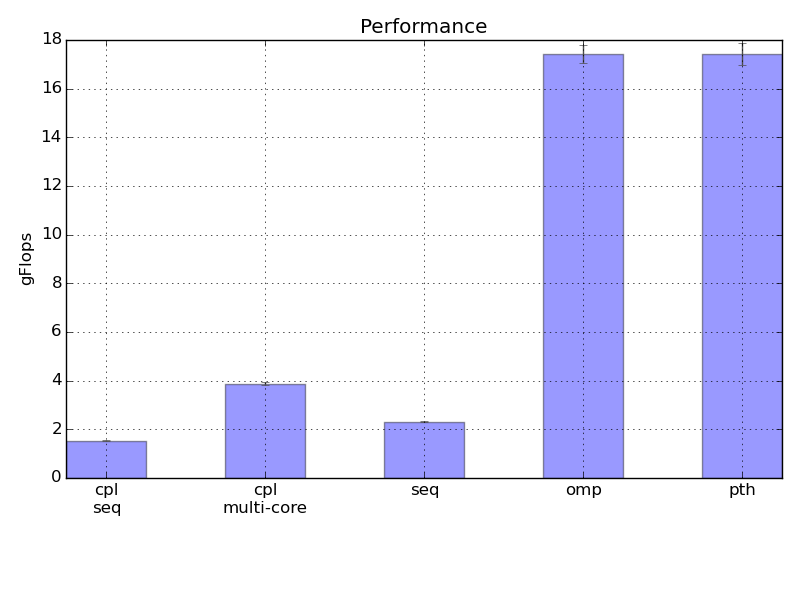
\includegraphics[width=0.75\columnwidth]{per_no_reductions.png} 

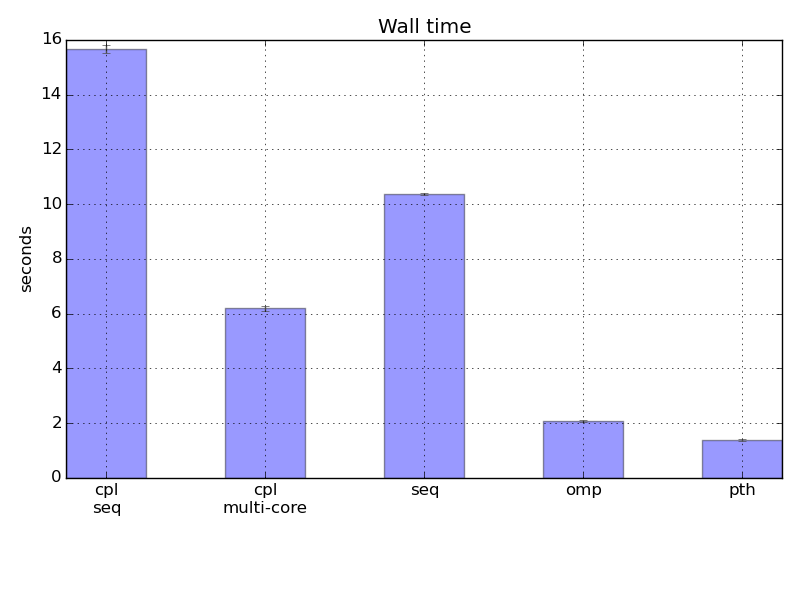
\includegraphics[width=0.75\columnwidth]{wt_no_reductions.png} 

Next, we consider a performance and walltime comparison overview with reductions.
We noticed that the performance of Chapel with or without reductions is almost the same which is a
result we didn't have on our earlier assignments concerning reductions. This might mean that the
parallelization of our main computation look might not be entirely optimized (which seems most likely), or that our reduction
implementation performs really well.

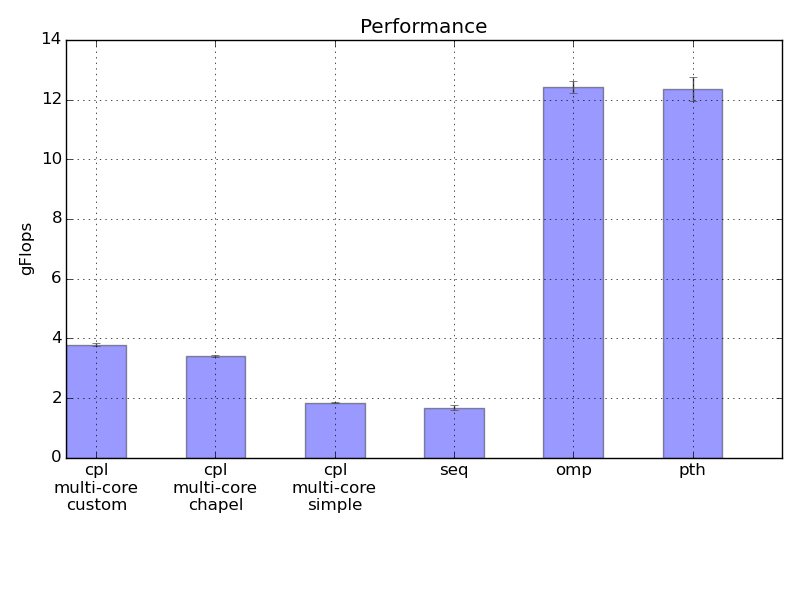
\includegraphics[width=0.75\columnwidth]{per_with_reductions.png} 

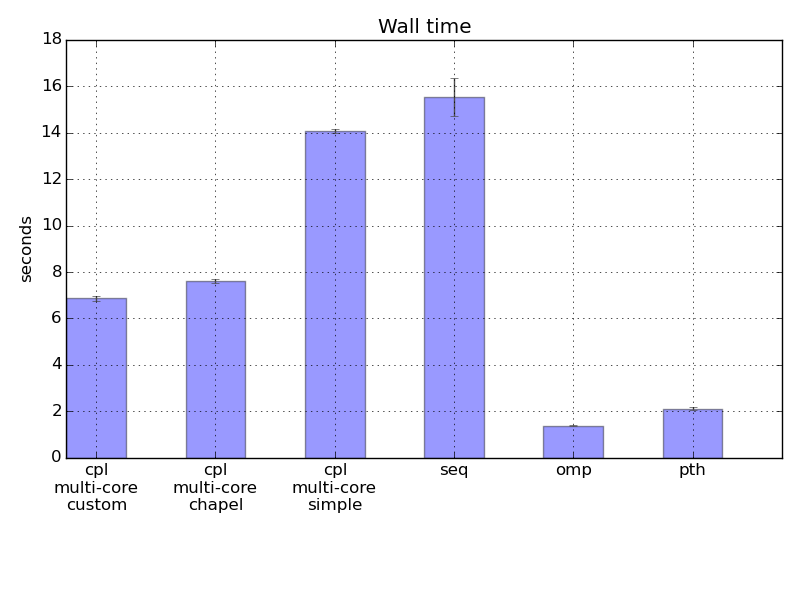
\includegraphics[width=0.75\columnwidth]{wt_with_reductions.png} 

These are graphs of different thread counts without reductions. We can clearly see the performance
peak when all 8 threads are used. We also notice poor performance (non linear) when we
specify 4 threads. 

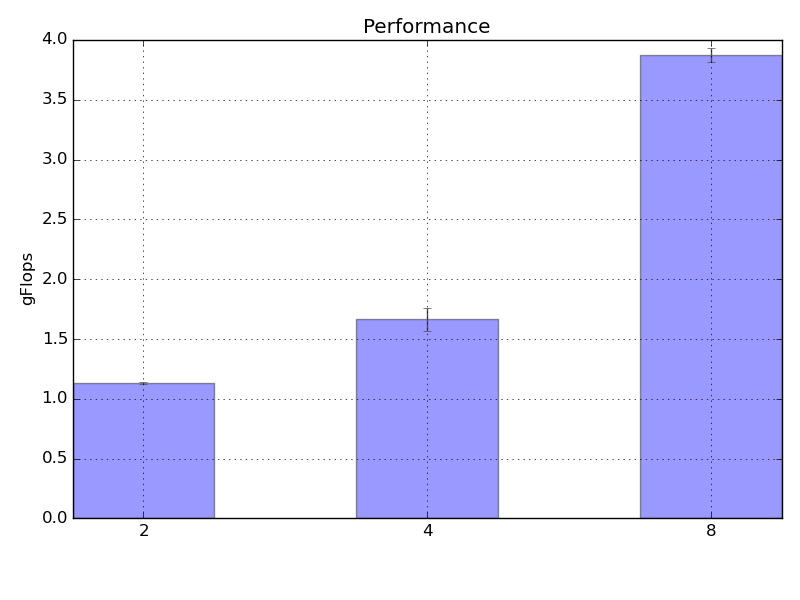
\includegraphics[width=0.75\columnwidth]{thread_without_reductions.png} 

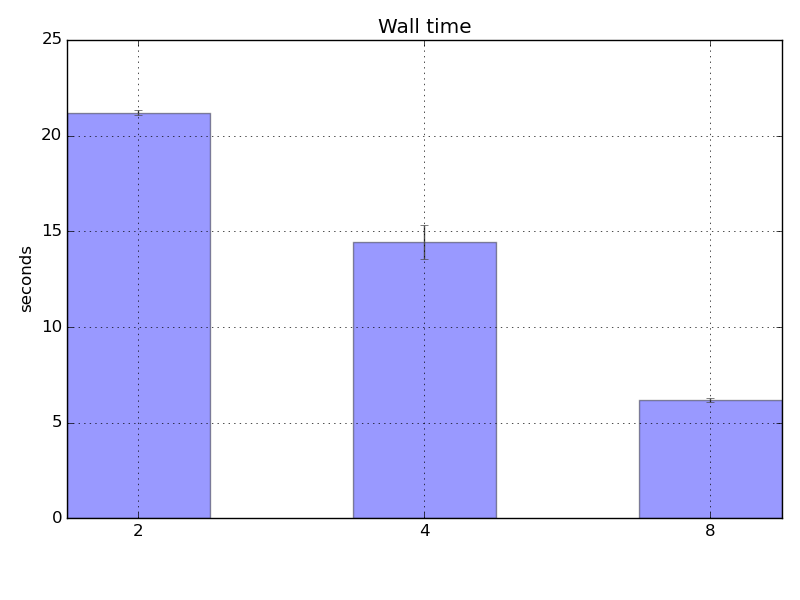
\includegraphics[width=0.75\columnwidth]{thread_without_reductions_wt.png} 

Finally, here are graphs of different thread counts with reductions. Note that the reduction method
used is our custom reduction, which as shown above performed best. As discussed, the speed is similar to the
speed obtained without reductions, for Chapel, which is quite impressive compared to our other attempts, but
probably indicates weird problems in our code.

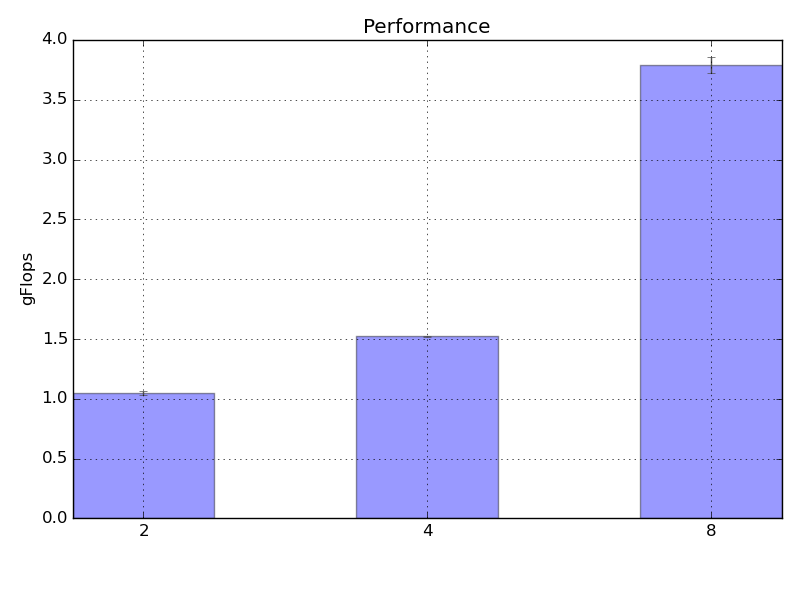
\includegraphics[width=0.75\columnwidth]{thread_with_reductions.png} 

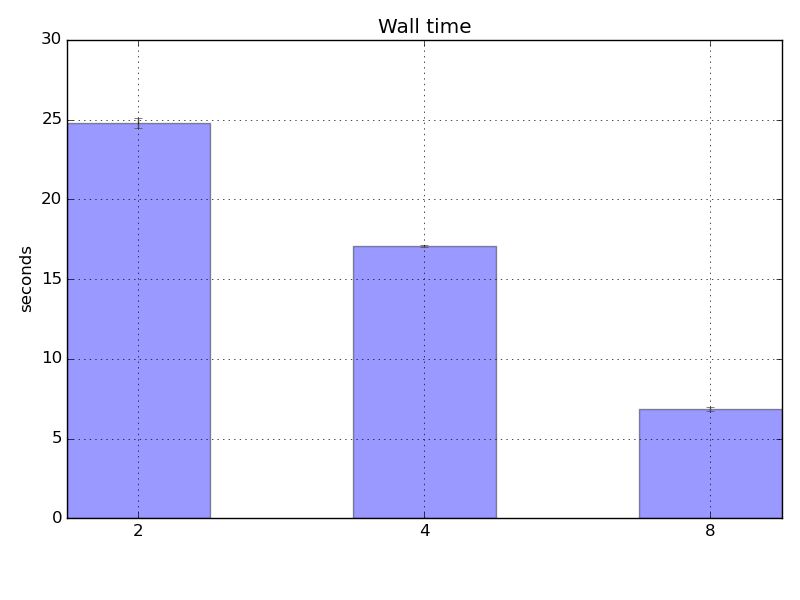
\includegraphics[width=0.75\columnwidth]{thread_with_reductions_wt.png} 

9 threads is far slower (unsurprising, due to HT), and 16 threads is still slower than 8, so we didn't
include those (yet) in our comparisons.

The experiments without reduction were made with the following parameters:

\begin{verbatim}
./heat -e 0.0 -i 2000 -k 2001
\end{verbatim}

and those with reduction:

\begin{verbatim}
./heat -e 0.0 -i 2000 -k 1
\end{verbatim}

\textbf{Improvements}

As discussed in the last session, large performance improvements can be obtained by using indexes into an
additional dimension, rather than swapping the entire contents of the arrays\cite{possdim}. We implemented this
using array aliasing as shown below, and obtained considerable speed improvements (which we won't discuss further
here, since it's beyond the deadline of the first sub-assignment).

\csnippet{extradim}{Using an additional dimension}

We also discovered that it is possible to include all reductions in the same custom reduction operator,
with (marginally) improved performance.

\end{homeworkProblem}

\begin{homeworkProblem}[Domain mapping | Chapel]

For the second part of the assignment, we were asked to use domain maps to run our Chapel code on multiple
nodes.

We were not successful in making this work well. Simply adding domain maps to our Chapel code results in a
large (more than an order of magnitude) performance decrease.

By printing \texttt{TwoBigDomains.dist} and \texttt{ProblemSpace.dist} (for example), it is possible to see
that the blocks get mapped to the locales in the intended fashion. For example, if we try a naive Block-based
distribution with a $1000 \times 1000$ matrix and two locales, it is split (as expected) into two parts, with
the extra dimension for our `swap trick' correctly not being distributed:

\begin{verbatim}
Block
-------
distributes: {1..1000, 1..1000, 0..0}
resulting in: 
  [(0, 0, 0)] locale 0 owns chunk: {..500, .., ..}
  [(1, 0, 0)] locale 1 owns chunk: {501.., .., ..}

Block
-------
distributes: {1..1000, 1..1000}
across locales: LOCALE0
LOCALE1
indexed via: {0..1, 0..0}
resulting in: 
  [(0, 0)] locale 0 owns chunk: {..500, ..}
  [(1, 0)] locale 1 owns chunk: {501.., ..}
\end{verbatim}

Compiling the Chapel code with \texttt{-sdebugBlockDist=true} enables debugging for the
block distribution, which reveals a huge number of Block distributions being created, but
otherwise gives little insight into our performance problems.

\end{homeworkProblem}

\begin{thebibliography}{9}

\bibitem{possdim}
  Raphael Poss,
  \emph{Pointer Operations in Chapel}.\\
  \texttt{https://sourceforge.net/p/chapel/mailman/message/27306614/}

\end{thebibliography}


\includepdf[pages={1}]{chapelaward.pdf}

\end{document}
